\subsubsection{Informazioni sul package}
\begin{figure}[h]
	\centering
	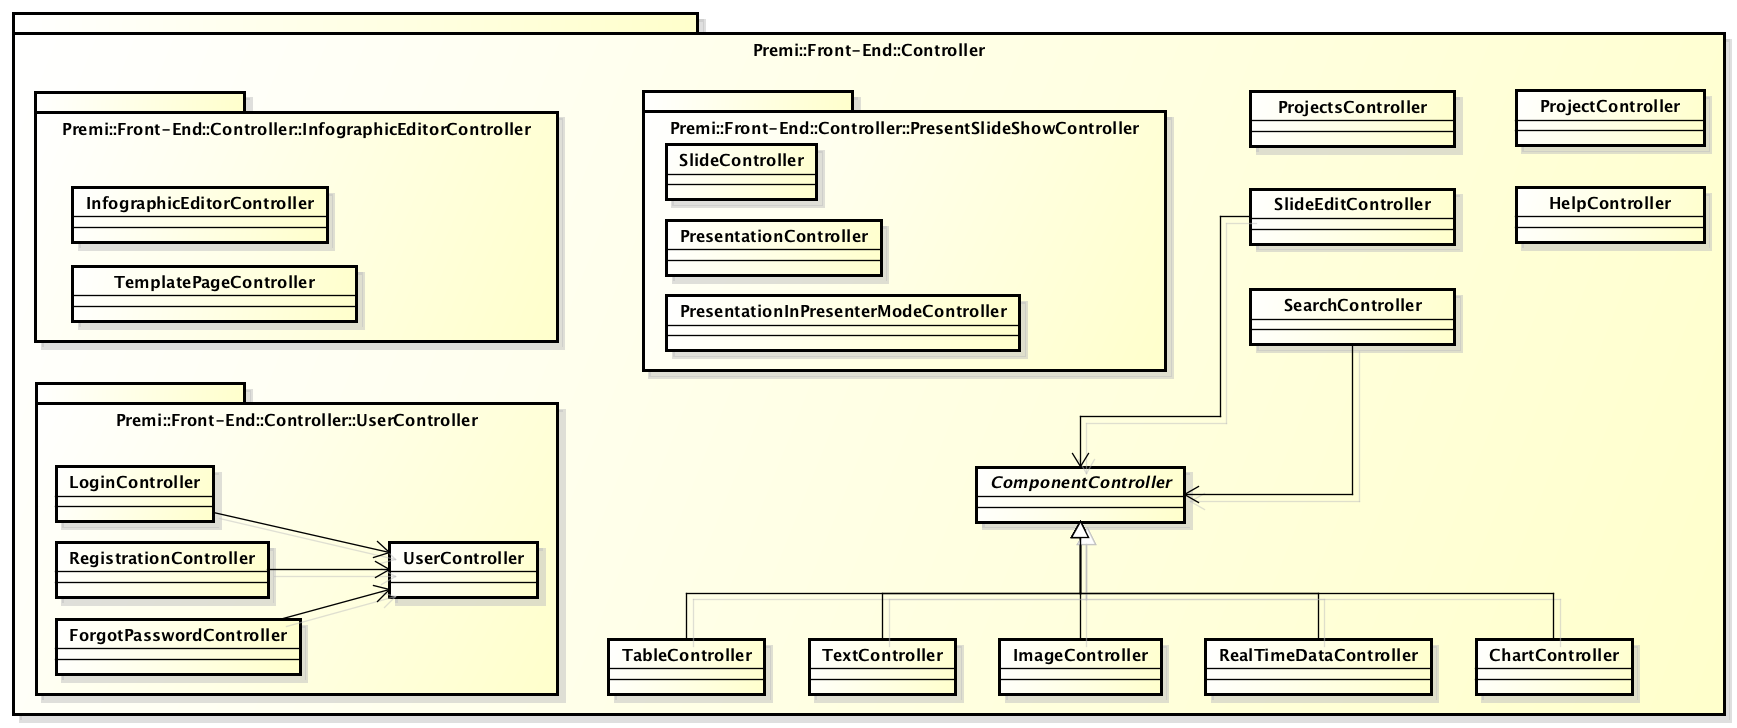
\includegraphics[width=1.0\linewidth]{img/front-end_controller}
	\caption[Premi::Front-End::Controllers]{Premi::Front-End::Controllers}
\end{figure}
\begin{itemize}
	\item \textbf{Descrizione}: Il package serve a far comunicare le view con il model in entrambe le direzioni ovvero rendere visibili gli aggiornamenti del model nella view e viceversa aggiornare il model con le informazioni provenienti dalla view.
	\item \textbf{Interazione con altri package}:
	\begin{itemize}
		\item Vi è un'interazione con il package Premi::Front-End::Views in quanto i controller sono utilizzati per iniziallizzare le view e per aggiornare il model del frontend con le modifiche avvenute in esse;
		\item Vi è un'interazione con il package Premi::Front-End::Model poiché in esso vengono depositati e prelevati i dati necessari alle view richieste;
		\item Vi è un'interazione con il package Premi::Front-End::Services responsabile del recupero e salvataggio delle informazioni e dell'invocazione di precise procedure dall'esterno mediante chiamate REST.
	\end{itemize}

\end{itemize}

\subsubsection{Classi contenute}
\begin{itemize}

	\item Premi::Front-End::Controllers::ProjectsController:
	\begin{itemize}
		\item \textbf{Descrizione}: classe con lo scopo di fornire le operazioni necessarie alla visualizzazione e gestione dei progetti relativi ad un utente.
		\item \textbf{Relazioni con altre classi}:
		\begin{itemize}
			\item Premi::Front-End::Services::ProjectService.
		\end{itemize}
	\end{itemize}
	\item  Premi::Front-End::Controllers::ProjectController:
	\begin{itemize}
		\item \textbf{Descrizione}: classe con lo scopo di fornire le operazioni necessarie alla gestione di un progetto.
		\item \textbf{Relazioni con altre classi}:
		\begin{itemize}
			\item Premi::Front-End::Services::ProjectService.
		\end{itemize}
	\end{itemize}
	\item  Premi::Front-End::Controllers::SlideEditorController:
	\begin{itemize}
		\item \textbf{Descrizione}: classe di suporto all'editor di una presentazione fornendo le operazioni necessarie alla composizione e modifica di una slide. Essa permette di assemblare e modificare una \gls{slide} e i metodi che effettueranno le operazioni sui componenti.
		\item \textbf{Relazioni con altre classi}:
		\begin{itemize}
			\item Premi::Front-End::Controllers::ComponentController;
			\item Premi::Front-End::Services::SlideService.
		\end{itemize}
	\end{itemize}
	\item  Premi::Front-End::Controllers::PresentationEditorController:
	\begin{itemize}
		\item \textbf{Descrizione}: classe con lo scopo di fornire le operazioni necessarie alla gestione dell'editor di una presentazione. Essa permette di assemblare e modificare una \gls{slide} e i metodi che effettueranno le operazioni sui componenti.
		\item \textbf{Relazioni con altre classi}:
		\begin{itemize}
			\item Premi::Front-End::Controllers::SlideEditorController;
			\item Premi::Front-End::Services::PresentationService.
		\end{itemize}
	\end{itemize}
	\item  Premi::Front-End::Controllers::InfographicEditorController:
	\begin{itemize}
		\item \textbf{Descrizione}: classe con lo scopo di fornire le operazioni necessarie alla gestione dell'editor di una inforgrafica. Essa permette di assemblare e modificare una \gls{slide} e i metodi che effettueranno le operazioni sui componenti.
		\item \textbf{Relazioni con altre classi}:
		\begin{itemize}
			\item Premi::Front-End::Services::InfographicService.
		\end{itemize}
	\end{itemize}
	\item  Premi::Front-End::Controllers::ComponentController:
	\begin{itemize}
		\item \textbf{Descrizione}: classe con lo scopo di fornire le operazioni necessarie alla gestione di un componente di una \gls{slide}.
	\end{itemize}
	\item  Premi::Front-End::Controllers::PresentationController:
	\begin{itemize}
		\item \textbf{Descrizione}: classe con lo scopo di fornire le operazioni necessarie alla gestione della visualizzazione di una presentazione. Essa permette di assemblare e configurare una presentazione e di rendere disponibile la visualizzazione in modalità classica o presentatore.
		\item \textbf{Relazioni con altre classi}:
		\begin{itemize}
			\item Premi::Front-End::Services::PresentationService.
		\end{itemize}
	\end{itemize}
	\item  Premi::Front-End::Controllers::LoginController:
	\begin{itemize}
		\item \textbf{Descrizione}: classe con lo scopo di fornire le operazioni necessarie all'autenticazione nel sistema.
		\item \textbf{Relazioni con altre classi}:
		\begin{itemize}
			\item Premi::Front-End::Services::AuthenticationService.
		\end{itemize}
	\end{itemize}
	\item  Premi::Front-End::Controllers::SignUpController:
	\begin{itemize}
		\item \textbf{Descrizione}: classe con lo scopo di fornire le operazioni necessarie alla registrazione di un nuovo utente nel sistema.
		\item \textbf{Relazioni con altre classi}:
		\begin{itemize}
			\item Premi::Front-End::Services::AuthenticationService.
		\end{itemize}
	\end{itemize}
	\item  Premi::Front-End::Controllers::SearchController:
	\begin{itemize}
		\item \textbf{Descrizione}: classe con lo scopo di fornire le operazioni necessarie alla ricerca di progetti e presentazioni mediante il titolo oppure il nome.
		\begin{itemize}
			\item Premi::Front-End::Services::ProjectService.
		\end{itemize}
	\end{itemize}
	\item  Premi::Front-End::Controllers::HelpController:
	\begin{itemize}
		\item \textbf{Descrizione}: classe con lo scopo di fornire le operazioni necessarie alla gestione dell'aiuto agli utenti sottoforma di tour\footnote{Un tour è una esplorazione guidata delle funzionalità basilari del sistema al fine di permettere all'utente di familiarizzare velocemente con esso.} e suggerimenti.
	\end{itemize}
\end{itemize}
\newpage
